\section{Setting}
    ”In the little town of Ohmville, electricity is in high demand. As director of the sole electric
    utility, it is your job to make sure all inhabitants are able to make coffee and play Nintendo
    Wii\texttrademark. You have at your disposal a certain amount of money, as well as the ability to build
    power plants and lay cables. You are the Watcher in the Night, the Bringer of Power and the
    Omnipotent Ottoman.”

\section{High Concept}
    The name for the game we settled on is Power Supply. It is in the construction and management 
    simulation genre and is inspired by games like SimCity, only in a more limited scope. You are 
    tasked with managing the delivery of electricity to buildings and factories in an area, while the 
    ultimate goal of the game is making money as the tycoon of the local power company, without going 
    bankrupt.

\section{Gameplay Description}

\subsection*{Player}
    The role of the player is to build powerplants to supply the buildings on the game map with power. 
    To do this the player has to connect the powerplants to the buildings with powerlines. Either directly
    or indirectly. Building powerplants and powerlines costs money. To earn money, the player has to supply
    power to the buildings on the map. If the inhabitants of a building does not get power then they will
    move out and abandon the building. If too many buildings become abandoned then the game is over.
    Abandoned buildings disappear from the game.

\subsection*{Powerplants}
    Powerplants can only supply a fixed amount of power to the connected buildings. If a powerplant is 
    unable to supply power to all the buildings on the map, the player has three options. The first option 
    is to build more powerplants. The second powerplant can then be connected to the buildings that the
    player wasn't previously able to supply with power. The second option is to upgrade the powerplant,
    so that it can deliver more power. This is supposed to be more cost effective in the short term, however
    it can become more expensive in the long run because of other important factors which will be brought
    up later. The final option is to demolish an already existing powerline and allow the powerplant to
    supply another building with power. This could be risky, as buildings that are not supplied with power
    will eventually become abandoned.

\subsection*{Powerlines}
    Powerlines is the way the player connects their powerplants to the buildings in need of power. This 
    can be done directly or indirectly. A direct connection is a connection between a powerplant and a 
    building in need of power. While an indirect connection is to connect a building with another building.
    Power from the powerplant then travels through the directly connected powerlines and continues down 
    the indirectly connected powerlines, supplying as many buildings as possible with power. Direct 
    connections are important, since buildings that are directly connected will receive power first.
    However you also have to consider the length of the powerline, as longer powerlines are more expensive
    to build than short powerlines. You can also tear down powerlines in order to supply other buildings
    with power.

    \begin{figure}[!ht]
    \centering
    \subfigure{
      
\includegraphics[scale=1]{pictures/coin.png}
    }
    \subfigure{
      
\includegraphics[scale=0.45]{pictures/factory_1_128.png}
    }
    \subfigure{
      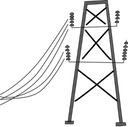
\includegraphics[scale=0.45]{pictures/pylon.png}
    }
    \caption{Game Elements: coin, power plant power line}
    \end{figure}


\subsection*{Buildings}
    Connecting buildings to powerplants is the main aspect of the gameplay. New buildings appear at 
    different locations on the map after a certain amount of time. Where the buildings appear and how 
    often they appear is random to a certain extent. There are also different types of buildings and 
    some of them require more power than others, for example factories. However buildings that require 
    more power also awards the player with more money. The player has to collect the money manually 
    by navigating the map and clicking on the buildings. If the buildings aren't connected to any 
    powerplants, they will eventually become abandoned and disappear from the map. If too many buildings 
    become abandoned it is game over.

    \begin{figure}[!ht]
    \centering

    \subfigure{
      
\includegraphics[scale=0.45]{pictures/house_2_128.png}
    }
    \subfigure{
      
\includegraphics[scale=0.45]{pictures/house_1_128.png}
    }
    \subfigure{
      
\includegraphics[scale=0.45]{pictures/house_3_128.png}
    }
    \subfigure{
      
\includegraphics[scale=0.45]{pictures/house_4_128.png}
    }
    \subfigure{
      
\includegraphics[scale=0.45]{pictures/factory_2_128.png}
    }
    \subfigure{
      
\includegraphics[scale=0.45]{pictures/company_1_128.png}
    }
    \caption{The buildings in the game}
    \end{figure}

\subsection*{Level and goal}
    Each level has a monetary goal that the player has to reach to proceed to
    the next level. At the end of a level, the player receives a highscore
    depending on how much time was spent on the level. When  the next level is
    reached the map is cleared and the player is presented with a new goal they
    have to reach. The map becomes larger and the sum of money the player has to
    earn is also increased. It will go faster and faster! How far does player
    get?
